%
% File acl2017.tex
%
%% Based on the style files for ACL-2015, with some improvements
%%  taken from the NAACL-2016 style
%% Based on the style files for ACL-2014, which were, in turn,
%% based on ACL-2013, ACL-2012, ACL-2011, ACL-2010, ACL-IJCNLP-2009,
%% EACL-2009, IJCNLP-2008...
%% Based on the style files for EACL 2006 by 
%%e.agirre@ehu.es or Sergi.Balari@uab.es
%% and that of ACL 08 by Joakim Nivre and Noah Smith

\documentclass[11pt,a4paper]{article}
\usepackage[hyperref]{acl2017}
\usepackage{times}
\usepackage{latexsym}
\usepackage{graphicx}
\usepackage{array}
\usepackage{makecell}
\usepackage{url}
\usepackage{lipsum}

%\aclfinalcopy % Uncomment this line for the final submission
%\def\aclpaperid{***} %  Enter the acl Paper ID here

%\setlength\titlebox{5cm}
% You can expand the titlebox if you need extra space
% to show all the authors. Please do not make the titlebox
% smaller than 5cm (the original size); we will check this
% in the camera-ready version and ask you to change it back.

\newcommand\BibTeX{B{\sc ib}\TeX}

\title{CMPUT 497 Project Report: \\ RAKE - Key Word Extraction Replication}

\author{Shouyang Zhou \\
  University of Alberta \\
  Edmonton, Alberta, Canada \\
  {\tt shoyang@ualberta.ca} \\\And
  Sharon Hains \\
  University of Alberta \\
  Edmonton, Alberta, Canada \\
  {\tt hains@ualberta.ca} \\\And
  Sharif Bakouny \\
  University of Alberta \\
  Edmonton, Alberta, Canada \\
  {\tt albakoun@ualberta.ca} \\}


\date{}

\begin{document}
\maketitle

\section{Introduction}

We aim to replicate the main evaluation from the article "Automatic Keyword Extraction from Individual Documents" by \citet{1}. This paper devises an unsupervised method for keyword extraction titled "RAKE" and compares it to a previous well performing unsupervised method called "TextRank". Details to follow in the evaluation section.

Keyword extraction is the automated process of extracting important words and phrases from a document. The importance of keyword extraction is in application, in information retrieval, feature engineering, and augmenting human classification tasks. At its most basic level, it helps humans process unstructured data in a more efficient and digestible manner. The importance of this replication study is to verify the results of \citet{1}, so we can be more confident in using RAKE as keyword extraction method. Confirming the results of RAKE testing is relevant as keyword extraction is a widely used application as discussed above. 

\subsection{Input-Output}
We will be using the dataset used in RAKE as our input, which is a set of abstracts, and processing the data. Our output will be a generation of keywords extracted from this set of abstracts. We will be comparing the number of correct keywords to extracted keywords, to determine how accurate our replication is to the original paper.

For the stoplist generation, our input will be the keywords from \citep{hulth-2003-improved} and the abstracts associated with each set of keywords. Our output will be a list of words generated to use as the stoplist. This list will be used for our RAKE testing. 

We will then be analyzing our output to create a table in the form of Table 1.2 in \citet{1}, please see the appendix for details. This will be a table comparing the performance of RAKE and TextRank variants (parameters) listing the metrics: extracted keywords (total, mean), correct keywords (total, mean), precision, recall, f-measure summarizing the replication-evaluation. 

\section{Related Work}

\citet{4} discusses TextRank, a graph-based ranking algorithm for keyword extraction, where the importance of a vertex (phrases) is decided by considering global information value of the phrase recursively computed from the entire graph (text). Implementing this algorithm goes as follows:

\begin{enumerate}
\item Identify text units and add them as vertices to the graph.
\item Edges of the graph are relations between text units.
\item Iterate the algorithm until convergence below a given threshold. 
\item Rank vertices based on their final scores (values).
\end{enumerate}   

The authors of TextRank evaluate their method to \citet{hulth-2003-improved} using the same dataset in RAKE, again, originating from \citet{hulth-2003-improved}.

We will not be recreating the results of \citet{hulth-2003-improved}, however as we are including their results in our evaluation for reference. \citet{1} describe their method where "Hulth (2003) compares the effectiveness of three term selection approaches: noun-phrase (NP) chunks, n-grams, and POS tags, with four discriminative features of these terms as inputs for automatic keyword extraction using a supervised machine-learning algorithm." \citet{1} noted difficulty in finding training materials used by \citet{hulth-2003-improved}.    

\section{Methodology}

The original paper “Automatic Keyword Extraction from Individual Documents” by \citet{1} is the primary work of interest. As mentioned, they evaluate their method "RAKE" and compare it with "TextRank" over two datasets. RAKE requires a set of phrase and content-word delimiters called a stoplist, a list of stopwords. Stop words are punctuation, numbers, conjunctions, and user specified terms which are used to delimit candidate keyword/phrases. 

A brief summary of the RAKE algorithm:
\begin{enumerate}
	\item Split the text into an array of words using the word delimiters.
	\item Split the array into sequences contiguous words using stop words and phrase delimiters.
	\item Candidate keywords are words in a sequence that are assigned the same position in the text. 
	\item Assign scores to each keyword candidate using ratio of degree to word-frequency. 
	\item Keywords that contain stop words:
	\begin{enumerate}
		\item A pair of candidate keywords must be adjoined at least twice in the text in the same order.
		\item Create a new keyword which contains the pair of keywords with interior stopwords between them.
		\item The new keyword’s score is the sum of the scores of its keywords components.
	\end{enumerate}
	\item The keywords of the text are the top T keywords from the keyword candidates list.
\end{enumerate}

\citet{1} also develops methods for stoplist generation. These stoplist generation methods leverage supervised datasets to generate dataset specific (thus domain specific) stoplists. 

A brief summary of the stoplist generation algorithm:
\begin{enumerate}
	\item With a manually selected list of keywords, find each keyword in the abstract.
	\item Look to the left and right words of the abstract.
	\item Count these words as 'adjacent words'.
	\item Iterate through the adjacent words list.
	\item For each abstract, find the count of each adjacency word, called the adjacency frequency.
	\item For each keyword, find the count of each adjacency word, called the keyword frequency.
	\item If the keyword frequency is higher than the adjacency frequency, remove this word from the adjacent words list.
	\item All items remaining in the list is our stoplist. 
\end{enumerate}

Once we have generated the keyword adjacency stoplist, we will test it with our implention of RAKE.

RAKE was compared to TextRank and seminal supervised learning methods \citep{hulth-2003-improved} over a dataset of human keyword annotated scientific paper abstracts originating from \citet{hulth-2003-improved}. The performance of RAKE depends on the stoplist used. RAKE was found to outperform all previously used keyword extraction algorithms in precision, efficiency and simplicity when using a domain specific stoplist. Using a generic stoplist, RAKE was found to be no worse performing than TextRank.

Since our initial proposal, we have found implementations of RAKE and TextRank in python (\citet{2}, \citet{3}). Since these are already available to us, we will replicate \citeapos{1} evaluation of the two using third party libraries. 

In essence, we will implement an evaluation script that feeds a dataset into these third party libraries to extract then aggregate the resultant metrics. This task will involve data collection, understanding the interface to the RAKE and TextRank implementations, preprocessing datasets to be fed into the two methods, and extracting and aggregating the results.

\section{Evaluation}

As our project is based on replicating the results of an article, we will evaluate the aggregate measures recorded as per the initial study and conduct an error analysis from samples from the replicating evaluation. 



\subsection{Data Sets \& Code Used}
For this reproduction we require three datasets:

\begin{enumerate}
\item \citet{hulth-2003-improved}'s dataset of human keyword annotated scientific paper abstracts.
\item Fox's Stoplist, a generic stopword-list.
\item The top 100 keywords generated provided from \citeapos{1}. The full list of words used in \citeapos{1} keyword adjacency stoplist was not available, so we are using what was provided in the paper to compare against our generated stoplist. 
\end{enumerate}  

As described in the methodology section, we also used Python implementations of RAKE and TextRank. 

We will be generating the Keyword Adjacency stoplist, which will be reproduced using the algorithm described in \citet{hulth-2003-improved}. To complete this, we will be tokenizing both each abstract and its keywords with spaCy's PhraseMatcher, and then completing the stoplist generation algorithm with this tokenized text. We will then test RAKE with our generated stoplist.

\subsection{Evaluation Metrics}

The measures reported in the original study by method were: number of extracted keywords, correct number of extracted keywords, precision, recall, and f-measure (f-score).  We will compare our recorded measures to that of the original study to what extent are \citeapos{1} results reproducible. We will consider \citeapos{1} results reproducible if the ordinal performance between RAKE and TextRank variants can be verified. 

\subsection{Results}
to do 

\lipsum[3]
\begin{table*}[t]
\scalebox{0.9}{
\centering
\begin{tabular}{>{\raggedright\arraybackslash}p{2.9cm}c c c c c c c }
	\hline
	                                         & \multicolumn{2}{c}{\makecell{Extracted \\ Keywords}} & \multicolumn{2}{c}{\makecell{Correct \\ Keywords}}       \\ \hline
	Method                                   &       Total        & Mean & Total            & Mean & Precision & Recall & F-Measure \\ \hline
	RAKE                                     &  \\
	\makecell[l]{KA stoplist \\(generated)}  & 8891               & 17.8 & 1962             & 3.9  & 23.8       & 40.7    & 28.7          \\
	Fox stoplist                             & 8152               & 16.3 & 2125             & 4.3  & 27.2       & 44.3    & 32.4          \\ \hline
	\makecell[l]{\citep{1} \\ RAKE}			 &  \\ 
	\makecell[l]{KA stoplist \\(\textit{df} $>$ 10)}     		  & 6052 & 12.1 			& 2037 & 4.1  		& 33.7    & 41.5    & 37.2       \\
	Fox stoplist     		 				 & 7893               & 15.8 & 2054             & 4.2  & 26         & 42.2    & 32.1      \\ \hline
	TextRank                                 &  \\
	\makecell[l]{Undirected, co-occ. \\window = 2} &                    &      &                  &      &           &        &           \\
	\makecell[l]{Undirected, co-occ. \\window = 3} &                    &      &                  &      &           &        &           \\ \hline
\end{tabular}
}
\end{table*} 

\subsection{Error Analysis}
Fusce maximus quam nec odio ullamcorper, consectetur aliquam mauris malesuada. Sed lacinia elit lectus, sed rutrum augue dictum non. Pellentesque tempor felis non mi hendrerit, vel sagittis nibh ultrices. Proin ullamcorper lorem in orci sollicitudin imperdiet. Maecenas iaculis convallis facilisis. Nunc lobortis eleifend lectus non aliquet. Sed sagittis, mauris cursus imperdiet venenatis, mi purus tincidunt massa, vel gravida enim tellus id dui. Sed lobortis tincidunt turpis. Aenean rhoncus sapien ex. Orci varius natoque penatibus et magnis dis parturient montes, nascetur ridiculus mus. Vivamus a rhoncus augue, quis sagittis nisi. Donec vulputate orci ut ultricies ornare. Vestibulum purus metus, aliquet in scelerisque vel, volutpat non sem. Donec hendrerit urna ante, non rutrum risus efficitur eget. Curabitur ligula felis, consectetur vitae ultricies id, condimentum et lectus. Morbi bibendum velit eget scelerisque dictum.

\section{Conclusion}

to do 

\section{Acknowledgments}

Teamwork Breakdown: Daniel wrote the code for re-creating the abstracts and the measures for tesing the output for TextRank and RAKE. Sharon wrote the code for generation the stoplist and found the datasets used from \citet{hulth-2003-improved}.
 

% include your own bib file like this:
%\bibliographystyle{acl}
%\bibliography{acl2017}
\bibliography{report}
\bibliographystyle{acl_natbib}

%\appendix

%\section{Table 1.2 from \citet{1}}
%\begin{figure}[b!]
%  \centering
%  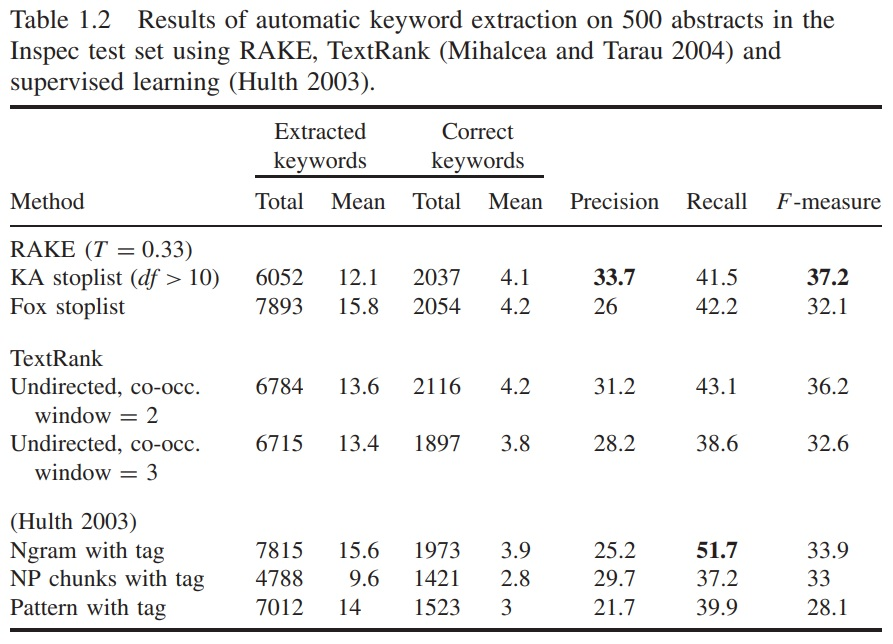
\includegraphics[width=\linewidth]{table1-2.jpg}
%  \caption{Table 1.2 from \citet{1}}
%\end{figure}


\end{document}
